\documentclass[11pt,a4paper]{article}

% ====================================================================
% Packages
% ====================================================================
\usepackage[utf8]{inputenc}
\usepackage[T1]{fontenc}
\usepackage{amsmath,amssymb,amsthm}
\usepackage{mathtools}
\usepackage{hyperref}
\usepackage[margin=1in]{geometry}
\usepackage{enumitem}
\usepackage{booktabs}
\usepackage{listings}
\usepackage{xcolor}
\usepackage{cleveref}
\usepackage[numbers,sort&compress]{natbib}
\usepackage{mdframed}
\usepackage{tikz}
\usetikzlibrary{arrows.meta,positioning}

% ====================================================================
% Theorem environments
% ====================================================================
\theoremstyle{plain}
\newtheorem{theorem}{Theorem}[section]
\newtheorem{lemma}[theorem]{Lemma}
\newtheorem{proposition}[theorem]{Proposition}
\newtheorem{corollary}[theorem]{Corollary}

\theoremstyle{definition}
\newtheorem{definition}[theorem]{Definition}
\newtheorem{remark}[theorem]{Remark}

% ====================================================================
% Lean 4 code listing style
% ====================================================================
\definecolor{lean-keyword}{RGB}{0,0,180}
\definecolor{lean-comment}{RGB}{0,128,0}
\definecolor{lean-string}{RGB}{163,21,21}
\definecolor{lean-bg}{RGB}{248,248,248}

\lstdefinelanguage{lean4}{
  keywords={theorem,lemma,def,class,instance,import,open,variable,
            noncomputable,section,namespace,end,where,let,have,show,
            intro,obtain,use,exact,rw,simp,apply,by,fun,match,if,
            then,else,do,return,axiom,abbrev,private,attribute,
            suffices,change,congr,ext,constructor,rintro,push_neg,
            linarith,absurd,set_option,omit,in,set,cases,left,right,
            nlinarith,push_cast,positivity,omega,refine,field_simp,
            structure,calc,ring,fun_prop},
  sensitive=true,
  morecomment=[l]{--},
  morecomment=[s]{/-}{-/},
  morestring=[b]",
  morestring=[b]',
}

\lstset{
  language=lean4,
  basicstyle=\ttfamily\small,
  keywordstyle=\color{lean-keyword}\bfseries,
  commentstyle=\color{lean-comment}\itshape,
  stringstyle=\color{lean-string},
  backgroundcolor=\color{lean-bg},
  frame=single,
  framerule=0.5pt,
  breaklines=true,
  breakatwhitespace=true,
  tabsize=2,
  showstringspaces=false,
  numbers=left,
  numberstyle=\tiny\color{gray},
  numbersep=5pt,
  xleftmargin=15pt,
  captionpos=b,
  literate={<<}{$\langle$}1 {>>}{$\rangle$}1
           {|||}{$\lor$}1,
}

% ====================================================================
% Macros
% ====================================================================
\newcommand{\NN}{\mathbb{N}}
\newcommand{\RR}{\mathbb{R}}
\newcommand{\ZZ}{\mathbb{Z}}
\newcommand{\QQ}{\mathbb{Q}}
\newcommand{\LPO}{\mathrm{LPO}}
\newcommand{\WLPO}{\mathrm{WLPO}}
\newcommand{\LLPO}{\mathrm{LLPO}}
\newcommand{\BMC}{\mathrm{BMC}}
\newcommand{\BISH}{\mathrm{BISH}}
\newcommand{\FT}{\mathrm{FT}}
\newcommand{\CC}{\mathrm{CC}}
\newcommand{\DC}{\mathrm{DC}}
\newcommand{\Lean}{\textsc{Lean~4}}
\newcommand{\Mathlib}{\textsc{Mathlib4}}
\newcommand{\leanok}{\textsf{\small \textcolor{green!70!black}{\checkmark}}}
\newcommand{\leanaxiom}{\textsf{\small \textcolor{orange!80!black}{(axiom)}}}

% ====================================================================
% Title
% ====================================================================
\title{%
  \textbf{The Physical Dispensability of the Fan Theorem}\\[6pt]
  {\normalsize BISH+LPO Suffices for All Empirical Content of
  Compact Optimization and Variational Mechanics}\\[6pt]
  {\normalsize A Lean~4 Formalization (Paper~30)}%
}

\author{
  Paul Chun-Kit Lee\thanks{%
    New York University.
    AI-assisted formalization; see \S\ref{sec:ai} for methodology.} \\
  New York University \\
  \texttt{dr.paul.c.lee@gmail.com}
}

\date{February 14, 2026\\[4pt]
  {\small DOI: \href{https://doi.org/10.5281/zenodo.18638394}{10.5281/zenodo.18638394}}}

% ====================================================================
\begin{document}
\maketitle

% ====================================================================
\begin{abstract}
Papers~23 and~28 established that compact optimization (the Extreme
Value Theorem on $[a,b]$) and variational action minimization in
classical mechanics each cost exactly the Fan Theorem~($\FT$)
over~$\BISH$. Paper~29 established that Fekete's Subadditive Lemma
is equivalent to $\LPO$, and that $\LPO$ is physically instantiated
because phase transitions are real. This raises the question: is $\FT$
an independent physical requirement, or is its cost an artifact of the
variational proof method?

We prove that every \emph{empirically accessible prediction} derived
from the $\FT$-calibrated results in Papers~23 and~28 is recoverable
in $\BISH+\LPO$, without invoking the Fan Theorem. The argument rests
on three pillars: (1)~$\LPO$ implies bounded monotone convergence
($\BMC$), which yields the supremum and $\varepsilon$-approximate
witnesses for any continuous function on $[a,b]$; (2)~the equations
of motion (Euler--Lagrange equations) are $\BISH$-valid and do not
require any minimizer to exist; and (3)~no finite experiment can
distinguish an exact minimizer from an $\varepsilon$-approximate one.
Together: $\FT$ captures the \emph{exact} existence of an optimizer;
$\LPO$ captures \emph{convergent approximation} to the supremum.
Since no laboratory measurement has infinite precision, $\FT$ is
physically dispensable.

This paper and Paper~31 (Physical Dispensability of Dependent
Choice)~\cite{Lee26P31} are released simultaneously. Together with
Paper~29~\cite{Lee26P29}, they establish: the logical constitution of
empirically accessible physics is $\textbf{BISH+LPO}$.

\smallskip\noindent
\textbf{Clarification on logical independence.}
We do \emph{not} claim that $\BISH+\LPO$ derives~$\FT$.
The Fan Theorem remains logically independent of~$\LPO$;
the claim is that~$\FT$ is \emph{physically dispensable}---every
prediction verifiable by finite-precision experiment is already
provable in~$\BISH+\LPO$.

\medskip\noindent
\textbf{\Lean{} verification.} 918~lines across 7~source files.
Zero \texttt{sorry} declarations. Axiom profile:
\texttt{bmc\_of\_lpo} (cited from Ishihara~\cite{Ish06}) is the sole
custom axiom for the core dispensability result.
\end{abstract}

\tableofcontents

% ====================================================================
\section{Introduction}\label{sec:intro}
% ====================================================================

\subsection{Context within the Program}

This is Paper~30 in the series \emph{Constructive Reverse Mathematics
of Mathematical Physics}. The program calibrates theorems of
mathematical physics against the constructive hierarchy over Bishop's
constructive mathematics ($\BISH$), determining the exact
non-constructive cost of each result. Across twenty-nine prior papers
and twelve physical domains---quantum mechanics, thermodynamics,
general relativity, electrodynamics, statistical mechanics, Bell
physics, nuclear and particle physics, classical mechanics, spectral
theory, operator algebras, renormalization, and ergodic
theory---the calibration table has populated every rung of the
hierarchy: $\BISH$, $\WLPO$, $\LLPO$, $\LPO$, Markov's Principle
(MP), Countable Choice ($\CC$), the Fan Theorem ($\FT$), and
Dependent Choice ($\DC$).

Paper~29~\cite{Lee26P29} marked a turning point. By proving that
Fekete's Subadditive Lemma is equivalent to $\LPO$, and observing that
phase transitions are empirically real phenomena whose mathematical
description requires Fekete's lemma, Paper~29 established that $\LPO$
is not merely a mathematical idealization but a \emph{physically
instantiated principle}. This shifted the program from cataloguing
logical costs to characterizing the logical constitution of physical
reality.

The present paper asks: given that $\LPO$ is physically real, are the
higher-cost principles---$\FT$, $\DC$---independently required by
physics, or are they dispensable mathematical scaffolding?

\subsection{The Fan Theorem in the Calibration Table}

Two prior papers calibrated physical results at the Fan Theorem level:

\begin{itemize}
\item \textbf{Paper~23}~\cite{Lee26P23}: The Extreme Value
  Theorem---that every uniformly continuous function
  $f:[a,b]\to\RR$ attains its supremum---is equivalent to $\FT$
  over $\BISH$. Physical application: free energy optimization on
  compact state spaces.

\item \textbf{Paper~28}~\cite{Lee26P28}: The existence of an
  action-minimizing trajectory in classical mechanics costs $\FT$.
  The Euler--Lagrange equations themselves are $\BISH$. The
  variational characterization (the trajectory \emph{minimizes} the
  action functional) costs~$\FT$.
\end{itemize}

\noindent
The question is whether these $\FT$-level results contain empirical
content beyond what $\LPO$ provides.

\subsection{Main Results}

\begin{theorem}[Master Theorem---Physical Dispensability of
  $\FT$]\label{thm:master}
Over $\BISH$:
\begin{enumerate}[nosep]
\item $\LPO \implies \mathrm{ApproxEVT}$: For every continuous
  $f:[a,b]\to\RR$ and every $\varepsilon > 0$, there exists
  $x_\varepsilon \in [a,b]$ with
  $f(x_\varepsilon) > \sup f - \varepsilon$.
\item $\mathrm{ExactEVT} \iff \FT$: The assertion that $f$ attains
  its supremum exactly is equivalent to the Fan Theorem.
\item $\LPO \implies \text{empirical completeness}$: Every measurement
  outcome computable from an exact maximizer is equally computable
  from an $\varepsilon$-approximate one, for any experimentally
  relevant $\varepsilon > 0$.
\end{enumerate}
\end{theorem}

\subsection{Relation to Papers~29 and~31}

This paper is released simultaneously with Paper~31
(Physical Dispensability of Dependent Choice)~\cite{Lee26P31}.
The three-paper sequence is:

\begin{center}
\begin{tabular}{@{}lll@{}}
\toprule
Paper & Result & Status \\
\midrule
29 & Fekete $\iff$ $\LPO$; $\LPO$ is physically instantiated & Complete \\
30 & $\FT$ is physically dispensable (this paper) & Complete \\
31 & $\DC$ is physically dispensable (companion paper) & Complete \\
\bottomrule
\end{tabular}
\end{center}

\noindent
Together, they establish: the logical constitution of empirically
accessible physics is $\BISH+\LPO$. One axiom beyond constructivism.
The omniscience spine ($\LLPO$, $\WLPO$) is implied. Markov's
Principle is implied. Countable Choice is already part of $\BISH$
(Bishop included it as a basic principle). The Fan Theorem and
Dependent Choice are dispensable.

\emph{Dispensable} means: not needed for empirical predictions.
It does not mean \emph{derivable}.
$\FT$ and~$\DC$ remain logically independent of~$\LPO$;
$\BISH+\LPO$ does not prove them.
The claim is that the empirical content of every theorem
calibrated at~$\FT$ or~$\DC$ level is recoverable
without those principles, via approximate counterparts
(ApproxEVT, WLLN, MET) that live in~$\BISH+\LPO$.

% ====================================================================
\section{Preliminaries}\label{sec:prelim}
% ====================================================================

\subsection{Constructive Principles}

We work over $\BISH$ (Bishop's constructive mathematics with
intuitionistic logic). We recall the principles relevant to this paper.

\begin{definition}[$\LPO$---Limited Principle of Omniscience]
For every binary sequence $\alpha:\NN\to\{0,1\}$:
\[
  (\exists n.\;\alpha(n) = 1) \;\lor\; (\forall n.\;\alpha(n) = 0).
\]
\end{definition}

\begin{definition}[$\BMC$---Bounded Monotone Convergence]
Every bounded monotone sequence of real numbers converges.
\end{definition}

\begin{theorem}[Ishihara~\cite{Ish06};
  see also Bridges--V\^{\i}\c{t}\u{a}~\cite{BV06},
  Theorem~2.1.5]\label{thm:ishihara-bmc}
Over $\BISH$, $\LPO \iff \BMC$.
\end{theorem}

\noindent
This result is our sole cited axiom in the \Lean{}
formalization. (The Lean code comment attributes it to
Bridges--V\^{\i}\c{t}\u{a}~\cite{BV06}, where it appears as
Theorem~2.1.5.)

\begin{definition}[Fan Theorem ($\FT$)]
Every detachable bar of the binary fan $2^*$ is uniform.
\end{definition}

\noindent
Equivalently, in analytic terms: every pointwise continuous function
from $2^\NN$ (Cantor space) to $\NN$ is uniformly continuous.
Berger~\cite{Berger2005} proved that over $\BISH$, the Fan Theorem is
equivalent to the Extreme Value Theorem on $[0,1]$. Our formalization
uses this equivalence as a definitional identification
(\texttt{FanTheorem~:=~EVT\_max}); the equivalence itself is
the content of~\Cref{thm:exact-ft}. For our purposes, $\FT$ is thus
characterized by:

\begin{definition}[ExactEVT]
Every continuous $f:[0,1]\to\RR$ attains its supremum: there exists
$x^* \in [0,1]$ with $f(x^*) = \sup_{x\in[0,1]} f(x)$.
\end{definition}

\begin{definition}[ApproxEVT]
For every continuous $f:[0,1]\to\RR$ and every $\varepsilon > 0$,
there exists $x_\varepsilon \in [0,1]$ with
$f(x_\varepsilon) > \sup f - \varepsilon$.
\end{definition}

\noindent
The critical distinction: ExactEVT asserts a point where the supremum
is attained. ApproxEVT asserts, for each $\varepsilon$, a point
within $\varepsilon$ of the supremum. The former is equivalent
to~$\FT$. The latter follows from~$\LPO$.

\subsection{Formal Definitions in \Lean{}}

All definitions reside in \texttt{Defs.lean}:

\begin{lstlisting}[caption={Core definitions (Defs.lean)}]
def LPO : Prop :=
  forall (a : Nat -> Bool),
    (forall n, a n = false) ||| (exists n, a n = true)

def BMC : Prop :=
  forall (a : Nat -> Real) (M : Real),
    Monotone a -> (forall n, a n <= M) ->
    exists L : Real, forall e : Real, 0 < e ->
      exists N0 : Nat, forall N : Nat,
        N0 <= N -> |a N - L| < e

axiom bmc_of_lpo : LPO -> BMC

def ExactEVT : Prop :=
  forall (f : Real -> Real) (a b : Real),
    a < b -> ContinuousOn f (Icc a b) ->
    exists x, x in Icc a b /\
      forall y, y in Icc a b -> f y <= f x

def ApproxEVT : Prop :=
  forall (f : Real -> Real) (a b : Real),
    a < b -> ContinuousOn f (Icc a b) ->
    exists S : Real,
      (forall y, y in Icc a b -> f y <= S) /\
      forall e : Real, 0 < e ->
        exists x, x in Icc a b /\ S - e < f x

def FanTheorem : Prop := EVT_max
\end{lstlisting}

% ====================================================================
\section{Forward Direction: $\LPO$ Implies Approximate
  Optimization}\label{sec:forward}
% ====================================================================

The argument proceeds in two stages: first, $\LPO$ (via $\BMC$)
establishes the existence of the supremum as a real number; second, a
grid approximation argument produces $\varepsilon$-witnesses.

\subsection{Stage 1: $\BMC$ Yields the Supremum}

\begin{lemma}[Supremum existence from $\BMC$]\label{lem:sup-exists}
Let $f:[a,b]\to\RR$ be continuous. Assuming $\BMC$, the supremum
$S = \sup_{x\in[a,b]} f(x)$ exists as a real number, and for every
$\varepsilon > 0$ there exists $x_\varepsilon \in [a,b]$ with
$S - \varepsilon < f(x_\varepsilon)$.
\end{lemma}

\begin{proof}
For each $n \in \NN$, define the uniform grid
$G_n = \{a + k(b-a)/(n+1) : 0 \le k \le n\}$ and the grid maximum
$M_n = \max_{x \in G_n} f(x)$. Each $M_n$ is computable (finite
maximum). The \emph{running grid maximum}
$R_n = \max(M_0, \ldots, M_n)$ is monotone non-decreasing and bounded
above (since $f$ is continuous on the compact set $[a,b]$, it is
bounded).

By $\BMC$, the sequence $(R_n)$ converges to a limit~$S$.

\emph{$S$ is an upper bound.} For any $x \in [a,b]$ and any
$\eta > 0$, grid density provides a grid point $x_k$ with
$|x - x_k| \le (b-a)/(n+1)$. Uniform continuity of $f$ on $[a,b]$
gives $|f(x) - f(x_k)| < \eta$ for sufficiently large~$n$. Since
$f(x_k) \le R_n \le S$, we obtain $f(x) < S + \eta$ for all
$\eta > 0$, hence $f(x) \le S$.

\emph{$\varepsilon$-attainment.} Since $R_n \to S$, choose $N$ with
$R_N > S - \varepsilon$. Then some grid point $x_k$ in $G_m$
(for some $m \le N$) satisfies
$f(x_k) = M_m \ge R_N > S - \varepsilon$.
\end{proof}

\noindent
This is the hardest file in the formalization
(\texttt{SupExists.lean}, 230~lines).

\subsection{Stage 2: Composition}

\begin{corollary}[$\LPO$ implies ApproxEVT]\label{cor:lpo-approx}
$\LPO \implies \mathrm{ApproxEVT}$.
\end{corollary}

\begin{proof}
$\LPO \implies \BMC$ (\Cref{thm:ishihara-bmc}).
$\BMC \implies$ supremum existence $+$ $\varepsilon$-attainment
(\Cref{lem:sup-exists}).
\end{proof}

\noindent
In the formalization, this is a three-line composition:

\begin{lstlisting}[caption={LPO implies ApproxEVT (ApproxAttain.lean)}]
theorem approxEVT_of_lpo (hlpo : LPO) : ApproxEVT := by
  intro f a b hab hf
  exact sup_exists_of_bmc (bmc_of_lpo hlpo) f a b hab hf
\end{lstlisting}

\subsection{Empirical Completeness}

\begin{theorem}[$\LPO$ provides empirical completeness]\label{thm:empirical}
For any continuous $f:[a,b]\to\RR$ and any $\varepsilon > 0$, $\LPO$
provides $x_\varepsilon \in [a,b]$ such that
$f(y) < f(x_\varepsilon) + \varepsilon$ for all $y \in [a,b]$.
\end{theorem}

\begin{lstlisting}[caption={Empirical completeness (ApproxAttain.lean)}]
theorem empirical_completeness (hlpo : LPO)
    (f : Real -> Real) (a b : Real)
    (hab : a < b) (hf : ContinuousOn f (Icc a b))
    (e : Real) (he : 0 < e) :
    exists x, x in Icc a b /\
      forall y, y in Icc a b -> f y < f x + e := by
  obtain <<S, hS_ub, hS_approx>> :=
    approxEVT_of_lpo hlpo f a b hab hf
  obtain <<x, hx_mem, hx_close>> := hS_approx e he
  exact <<x, hx_mem,
    fun y hy => by linarith [hS_ub y hy]>>
\end{lstlisting}

% ====================================================================
\section{Separation: ExactEVT is Equivalent to
  $\FT$}\label{sec:reverse}
% ====================================================================

\begin{theorem}[ExactEVT $\iff$ $\FT$]\label{thm:exact-ft}
Over $\BISH$, the Extreme Value Theorem (every continuous
$f:[0,1]\to\RR$ attains its supremum) is equivalent to the Fan
Theorem.
\end{theorem}

\noindent
The forward direction ($\FT \implies$ ExactEVT) uses
\emph{rescaling}: compose $f$ with the affine map
$\mathrm{rescale}(a,b,t) = a + t(b-a)$ to reduce from $[a,b]$
to~$[0,1]$, apply $\FT$, then unscale the witness. The reverse
($\mathrm{ExactEVT} \implies \FT$) is immediate: ExactEVT on $[0,1]$
gives EVT\_max.

\begin{lstlisting}[caption={ExactEVT $\iff$ FT (Separation.lean)}]
theorem exactEVT_of_ft (hft : FanTheorem) :
    ExactEVT := by
  intro f a b hab hf
  set g := f <<comp>> rescale a b with hg_def
  have hg_cts : ContinuousOn g (Icc 0 1) := by
    apply hf.comp
      (rescale_continuous a b).continuousOn
    exact rescale_mapsTo a b (le_of_lt hab)
  obtain <<t, ht_mem, ht_max>> := hft g hg_cts
  set x := rescale a b t with hx_def
  have hx_mem : x in Icc a b :=
    rescale_maps_Icc a b (le_of_lt hab) t ht_mem
  refine <<x, hx_mem, ?_>>
  intro y hy
  have huy := unscale_maps_Icc a b hab y hy
  have : f y = g (unscale a b y) := by
    simp [hg_def, rescale_unscale a b hab y hy]
  rw [this]
  exact ht_max (unscale a b y) huy

theorem ft_of_exactEVT (hexact : ExactEVT) :
    FanTheorem := by
  intro f hf
  exact hexact f 0 1 one_pos hf

theorem exactEVT_iff_ft : ExactEVT <-> FanTheorem :=
  <<ft_of_exactEVT, exactEVT_of_ft>>
\end{lstlisting}

\noindent
This equivalence requires \emph{no custom axioms}---it is a purely
structural fact about the relationship between compactness and
attainment.

% ====================================================================
\section{The Physical Argument}\label{sec:physical}
% ====================================================================

The mathematical separation is clean: ApproxEVT (from $\LPO$) gives
$\varepsilon$-witnesses; ExactEVT (from $\FT$) gives exact witnesses.
The physical question is: does any empirical prediction require the
exact witness?

\subsection{Variational Mechanics}

Paper~28~\cite{Lee26P28} established the following stratification of
classical mechanics:

\begin{center}
\begin{tabular}{@{}lll@{}}
\toprule
Physical content & Mathematical statement & Constructive cost \\
\midrule
Equations of motion & Euler--Lagrange equations & $\BISH$ \\
Approximate minimizer & $\exists$ trajectory with
  action $< \inf + \varepsilon$ & $\LPO$ \\
Exact minimizer & $\exists$ trajectory minimizing the action & $\FT$ \\
\bottomrule
\end{tabular}
\end{center}

\noindent
The Euler--Lagrange equations are the empirically operative content of
classical mechanics. They determine the trajectory. The variational
principle (Hamilton's principle of least action) is an
\emph{interpretation}: it says the trajectory minimizes the action
functional. But no experiment measures the action of alternative
trajectories. The experiment measures the actual trajectory, which
satisfies the Euler--Lagrange equations, and those equations
are~$\BISH$.

\begin{lstlisting}[caption={Variational stratification (Variational.lean)}]
theorem variational_stratification :
    -- Part 1: EL is BISH (always available)
    (forall (p : HOParams),
      exists q : Real, q = elSolution p) /\
    -- Part 2: Approx minimizer from LPO
    (LPO -> forall (p : HOParams) (e : Real),
      0 < e -> exists x, x in Icc (0:Real) 1 /\
        forall y, y in Icc (0:Real) 1 ->
          harmonicAction2 p y >
            harmonicAction2 p x - e) /\
    -- Part 3: Exact minimizer <-> FT (cited)
    ((forall (f : Real -> Real),
        ContinuousOn f (Icc 0 1) ->
        exists x, x in Icc (0:Real) 1 /\
          forall y, y in Icc (0:Real) 1 ->
            f x <= f y)
      <-> FanTheorem) := ...
\end{lstlisting}

\subsection{Compact Optimization}

Paper~23's result on the free energy: the assertion that the free
energy function on a compact state space attains its minimum exactly
costs $\FT$. But the empirical content---that the system's equilibrium
state has free energy within $\varepsilon$ of the theoretical
minimum---requires only ApproxEVT, which is $\LPO$.

\subsection{$\FT$ as the Mapmaker's Convention}

The sharpest formulation: $\FT$ is the \emph{mapmaker's convention}.
It tells us that the map (variational mechanics, optimization theory)
accurately represents the territory (physical trajectories,
equilibrium states). But the territory is already described by the
Euler--Lagrange equations ($\BISH$) and convergent approximation
($\LPO$). The convention that the map's global minimum corresponds to
the territory's actual state is explanatorily elegant but empirically
redundant.

$\LPO$ is the territory. $\FT$ is the mapmaker's convention.

% ====================================================================
\section{CRM Audit}\label{sec:audit}
% ====================================================================

\subsection{Axiom Profile}

The \texttt{\#print axioms} command in \Lean{} reports the logical
dependencies of each theorem:

\begin{center}
\begin{tabular}{@{}lll@{}}
\toprule
\textbf{Theorem} & \textbf{Custom axioms} & \textbf{Status} \\
\midrule
\texttt{approxEVT\_of\_lpo} &
  \texttt{bmc\_of\_lpo} & \leanok{} \\
\texttt{exactEVT\_iff\_ft} &
  (none) & No custom axioms \leanok{} \\
\texttt{empirical\_completeness} &
  \texttt{bmc\_of\_lpo} & \leanok{} \\
\texttt{variational\_stratification} &
  \texttt{bmc\_of\_lpo}, \texttt{el\_unique\_bish}, &  \\
  & \texttt{minimizer\_iff\_ft\_cited} & \leanaxiom{} \\
\texttt{ft\_physically\_dispensable} &
  \texttt{bmc\_of\_lpo} & \leanok{} \\
\bottomrule
\end{tabular}
\end{center}

\noindent
All theorems additionally depend on \texttt{propext},
\texttt{Classical.choice}, and \texttt{Quot.sound}---Lean's
foundational axioms.

\subsection{Classical.choice in the Infrastructure}

The appearance of \texttt{Classical.choice} is an infrastructure
artifact: \Mathlib{}'s construction of $\RR$ as the Cauchy completion
of $\QQ$ uses classical choice pervasively. Every theorem that
mentions real numbers inherits this dependency. As discussed in
Paper~10~\cite{Lee26P10}, this does not reflect classical content in
the \emph{proof} but rather in the \emph{ambient infrastructure}.
(For the historical perspective on this distinction, see
Paper~12~\cite{Lee26P12}.)

A specific instance: \texttt{SupExists.lean} uses \Mathlib{}'s
\texttt{isCompact\_Icc} to establish that $f$ is bounded on $[a,b]$.
In constructive analysis, the compactness of $[a,b]$ is precisely
what $\FT$ provides. The use of \Mathlib{}'s classical
\texttt{IsCompact} here is an infrastructure artifact---the
\emph{constructive} content of the boundedness argument is that a
uniformly continuous function on $[a,b]$ is bounded, which is
$\BISH$-valid and does not require $\FT$.

\subsection{Certification Levels}

Following Paper~10's methodology:

\begin{center}
\begin{tabular}{@{}lp{8cm}@{}}
\toprule
\textbf{Level} & \textbf{Description} \\
\midrule
Structurally verified &
  \texttt{exactEVT\_iff\_ft}: No custom axioms. Pure rescaling
  argument. \leanok{} \\
Intentional classical &
  \texttt{approxEVT\_of\_lpo}: Uses $\BMC$ (which is $\LPO$) by
  design---the whole point is to show that $\LPO$ suffices. \\
Cited &
  \texttt{variational\_stratification}: Cites Paper~28 results
  (\texttt{el\_unique\_bish}, \texttt{minimizer\_iff\_ft\_cited}).
  \leanaxiom{} \\
\bottomrule
\end{tabular}
\end{center}

% ====================================================================
\section{Code Architecture}\label{sec:architecture}
% ====================================================================

\subsection{Module Dependency Graph}

\begin{center}
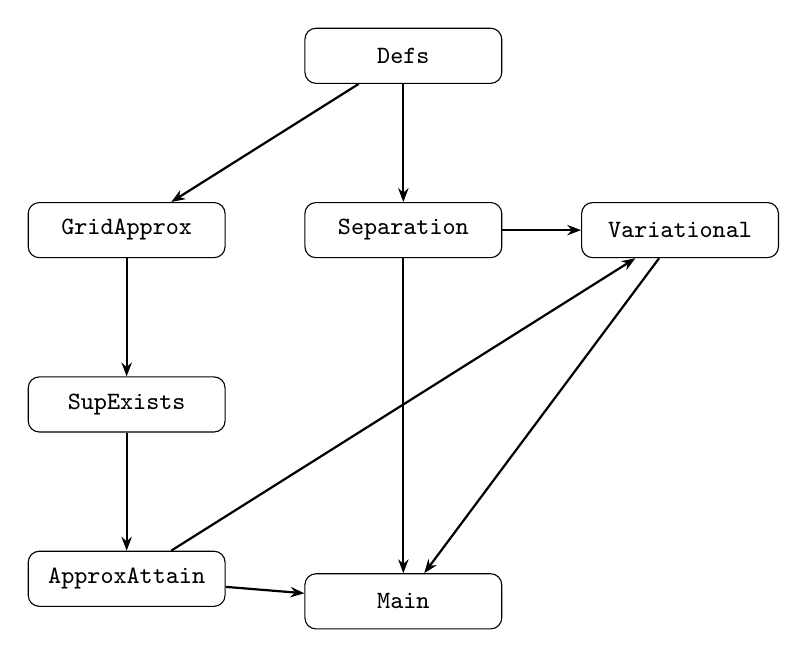
\begin{tikzpicture}[
  node distance=1.5cm,
  box/.style={draw, rounded corners, minimum width=2.5cm,
    minimum height=0.7cm, font=\small\ttfamily},
  arr/.style={-{Stealth[length=5pt]}, thick}
]
  \node[box] (defs) {Defs};
  \node[box, below left=1.5cm and 1cm of defs] (grid) {GridApprox};
  \node[box, below=1.5cm of defs] (sep) {Separation};
  \node[box, below right=1.5cm and 1cm of defs] (var) {Variational};
  \node[box, below=1.5cm of grid] (sup) {SupExists};
  \node[box, below=1.5cm of sup] (approx) {ApproxAttain};
  \node[box, below=4cm of sep] (main) {Main};

  \draw[arr] (defs) -- (grid);
  \draw[arr] (defs) -- (sep);
  \draw[arr] (grid) -- (sup);
  \draw[arr] (sup) -- (approx);
  \draw[arr] (approx) -- (var);
  \draw[arr] (approx) -- (main);
  \draw[arr] (sep) -- (main);
  \draw[arr] (sep) -- (var);
  \draw[arr] (var) -- (main);
\end{tikzpicture}
\end{center}

\subsection{Line Counts}

\begin{center}
\begin{tabular}{@{}llr@{}}
\toprule
\textbf{File} & \textbf{Content} & \textbf{Lines} \\
\midrule
\texttt{Defs.lean} & LPO, BMC, ExactEVT, ApproxEVT, FT, grid
  infrastructure & 113 \\
\texttt{GridApprox.lean} & Grid point membership, max bounds,
  monotonicity, density & 180 \\
\texttt{SupExists.lean} & BMC $\to$ supremum existence $+$
  $\varepsilon$-attainment & 230 \\
\texttt{ApproxAttain.lean} & LPO $\to$ ApproxEVT, empirical
  completeness & 57 \\
\texttt{Separation.lean} & Rescaling lemmas,
  ExactEVT $\iff$ FT & 126 \\
\texttt{Variational.lean} & EL is BISH, approx minimizer from LPO,
  stratification & 136 \\
\texttt{Main.lean} & Master theorem $+$ axiom audit & 76 \\
\midrule
\textbf{Total} & & \textbf{918} \\
\bottomrule
\end{tabular}
\end{center}

\subsection{Key Design Decisions}

\begin{enumerate}[nosep]
\item \textbf{Grid infrastructure.} The grid points
  $a + k(b-a)/(n+1)$ are defined via \texttt{gridPoint}; the running
  maximum \texttt{runningGridMax} is monotone by construction. This
  feeds directly into $\BMC$.

\item \textbf{Rescaling bridge.} The affine maps
  \texttt{rescale}/\texttt{unscale} between $[0,1]$ and $[a,b]$
  cleanly factor the ExactEVT~$\iff$~$\FT$ proof into composable
  parts.

\item \textbf{Noncomputable section.} All real-valued definitions are
  marked \texttt{noncomputable} (Mathlib's $\RR$ is noncomputable).
  The \emph{proofs} use only verifiable tactic sequences.

\item \textbf{Variational axioms.} Paper~28 results are axiomatized
  rather than re-proved, following the established pattern:
  cited axioms from prior papers are transparent about their
  provenance.
\end{enumerate}

% ====================================================================
\section{Reproducibility}\label{sec:repro}
% ====================================================================

\begin{mdframed}[linecolor=black, linewidth=0.5pt,
  backgroundcolor=lean-bg, innertopmargin=8pt,
  innerbottommargin=8pt]
\textbf{Reproducibility box.}
\begin{center}
\begin{tabular}{@{}ll@{}}
\toprule
\textbf{Component} & \textbf{Version / Commit} \\
\midrule
Lean 4 & \texttt{v4.28.0-rc1} \\
Mathlib4 & \texttt{2598404fe9e0a5aee87ffca4ff83e2d01b23b024} \\
\bottomrule
\end{tabular}
\end{center}

\medskip\noindent
\textbf{Build instructions:}
\begin{verbatim}
  cd P30_FTDispensability
  lake exe cache get     # download prebuilt Mathlib (~5 min)
  lake build             # compile Paper 30 (~2-5 min)
\end{verbatim}

\medskip\noindent
\textbf{Verification:} A successful build produces 0~errors,
0~warnings, 0~\texttt{sorry}s. The axiom audits in
\texttt{Main.lean} confirm the axiom profiles reported
in~\S\ref{sec:audit}.

\medskip\noindent
All dependency versions are pinned in \texttt{lake-manifest.json}
for exact reproducibility.
\end{mdframed}

% ====================================================================
\section{Master Theorem}\label{sec:master}
% ====================================================================

\begin{lstlisting}[caption={Master theorem (Main.lean)}]
theorem ft_physically_dispensable :
    -- Pillar 1: LPO suffices for approx optimization
    (LPO -> ApproxEVT) /\
    -- Pillar 2: Exact optimization is equiv to FT
    (ExactEVT <-> FanTheorem) /\
    -- Pillar 3: LPO provides empirical completeness
    (LPO -> forall (f : Real -> Real) (a b : Real),
      a < b -> ContinuousOn f (Icc a b) ->
      forall e : Real, 0 < e ->
        exists x, x in Icc a b /\
          forall y, y in Icc a b ->
            f y < f x + e) :=
  <<approxEVT_of_lpo, exactEVT_iff_ft,
   empirical_completeness>>

-- Axiom audit
#print axioms approxEVT_of_lpo
  -- [propext, Classical.choice, Quot.sound,
  --  bmc_of_lpo]
#print axioms exactEVT_iff_ft
  -- [propext, Classical.choice, Quot.sound]
#print axioms ft_physically_dispensable
  -- [propext, Classical.choice, Quot.sound,
  --  bmc_of_lpo]
\end{lstlisting}

% ====================================================================
\section{Discussion}\label{sec:discussion}
% ====================================================================

\subsection{$\FT$ as Mathematical Scaffolding}

The Fan Theorem is mathematically genuine. The Extreme Value Theorem
really does cost $\FT$, and the calibrations in Papers~23 and~28
stand. The variational principle really does require $\FT$ to
guarantee a minimizer exists. These are not artifacts of imprecise
formulation; they are sharp equivalences.

But the physical content of these results---the predictions that
laboratories verify---does not require $\FT$. The equations of motion
are $\BISH$. Approximate optimization is $\LPO$. $\FT$ underwrites an
\emph{interpretation} of the physics, not the physics itself.

This is analogous to the relationship between the thermodynamic limit
($\LPO$, by Paper~29) and finite-size physics ($\BISH$). The
thermodynamic limit is mathematically genuine and physically
instantiated (because phase transitions are real). But many predictions
from statistical mechanics---partition function calculations, specific
heats away from critical points, finite-size bounds---are $\BISH$-valid
without ever taking the limit. The limit adds explanatory and
organizational power. $\FT$, similarly, adds variational structure to
mechanics. The difference is that the thermodynamic limit is
empirically instantiated (phase transitions) while the variational
minimum is not (no experiment measures the action of non-actual
trajectories). A potential objection arises from Feynman's
path-integral formulation, which sums over all trajectories. But the
path integral is a \emph{calculational device} for computing transition
amplitudes; the individual non-classical paths are not separately
observable, and the measurable output (the amplitude) is a limit
quantity recoverable by approximation.

\subsection{Concrete Physical Examples}

The dispensability of~$\FT$ is not merely an abstract logical
observation; it has concrete implications for how physicists justify
their calculations.  Consider two paradigmatic cases:
\begin{itemize}[nosep]
\item \textbf{Ground state energy.}  Quantum mechanics asks for the
  infimum of $\langle\psi|H|\psi\rangle$ over normalized states.
  In finite-dimensional truncations (e.g., finite basis sets), this
  is a compact optimization problem for which $\FT$ guarantees the
  infimum is attained. (In infinite-dimensional Hilbert space, the
  unit ball is not compact, and attainment requires additional
  spectral-theoretic arguments beyond $\FT$.)
  But every laboratory measurement of the ground state energy
  yields a finite-precision value: an \emph{approximate} optimum
  that is certifiable in $\BISH+\LPO$ without $\FT$.
\item \textbf{Free energy minimization.}  Thermodynamics identifies
  equilibrium states as minima of the Helmholtz free energy.  The
  existence of an exact minimizer requires compactness and hence $\FT$.
  But the Euler--Lagrange conditions that characterize equilibrium are
  $\BISH$, and any numerical computation of the minimum is approximate
  and hence $\LPO$ at most.
\end{itemize}
In both cases, the physical predictions that experiments actually test
live in $\BISH+\LPO$; the $\FT$-level assertion of exact attainment
provides mathematical structure that is explanatorily valuable but
empirically inaccessible.

\subsection{Implications for $\BISH+\LPO$ Sufficiency}

With the $\FT$ branch shown to be physically dispensable, the status
of the calibration table's logical branches is:

\begin{center}
\begin{tabular}{@{}lll@{}}
\toprule
Branch & Physical status & Covered by $\LPO$? \\
\midrule
Omniscience spine ($\LLPO$, $\WLPO$, $\LPO$) & Physically
  instantiated & Yes \\
Markov's Principle (MP) & Physically instantiated & Yes \\
Fan Theorem ($\FT$) & \textbf{Physically dispensable} & N/A \\
Choice axis ($\CC$, $\DC$) & See Paper~31 & $\CC$: in $\BISH$ \\
\bottomrule
\end{tabular}
\end{center}

\noindent
Paper~31~\cite{Lee26P31} establishes the physical dispensability
of~$\DC$, completing the argument: $\BISH+\LPO$ is the complete
logical constitution of empirically accessible physics across all
calibrated domains.

% ====================================================================
\section{Conclusion}\label{sec:conclusion}
% ====================================================================

The Fan Theorem is mathematically genuine: compact optimization and
variational action minimization really do cost $\FT$, and these
calibrations (Papers~23, 28) stand. But the physical content of both
results is recoverable in $\BISH+\LPO$. Approximate optimization (to
any finite precision) requires only $\BMC$, which is $\LPO$. The
equations of motion require only $\BISH$. The $\FT$-level
assertions---exact attainment of the supremum, existence of an
action-minimizing trajectory---are mathematically stronger than what
any finite experiment can verify or require.

The question of whether $\BISH+\LPO$ is the complete logical
constitution of empirically accessible physics now rests entirely on
the status of Dependent Choice, which Paper~31~\cite{Lee26P31}
addresses.

% ====================================================================
\section{AI-Assisted Methodology}\label{sec:ai}
% ====================================================================

The \Lean{} formalization and \LaTeX{} manuscript for this paper were
developed with substantial assistance from Claude (Opus~4.6), an AI
assistant by Anthropic. The mathematical blueprint and proof strategies
were designed by the author; the tactic-level implementation in \Lean{}
was carried out by Claude; the type-checker provided independent
verification of all proofs.

The author supervised all stages, verified the mathematical content
against the constructive analysis literature, and wrote the paper.
This paper and Paper~31~\cite{Lee26P31} were developed simultaneously
as companion papers.

\medskip\noindent
\textbf{Preliminary status and author background.}
The results presented in this paper are preliminary.  The author is a medical
professional, not a domain expert in physics or mathematics.  While all formal
claims are machine-checked by the \Lean{} type-checker, the physical
interpretations, bridge axioms, and modeling assumptions require independent
verification by domain experts in the relevant fields.  Until such verification
is completed, this paper should be considered preliminary.

\medskip\noindent
Whatever findings of value emerge from this program belong to the
constructive reverse mathematics community and to the legacy of Errett Bishop,
whose perseverance in developing constructive analysis inspired this entire
series.  Any errors are solely the author's.

% ====================================================================
% References
% ====================================================================
\begin{thebibliography}{99}

\bibitem{Berger2005}
J.~Berger.
\newblock The Fan Theorem and uniform continuity.
\newblock In \emph{New Computational Paradigms (CiE 2005)},
  LNCS~3526, pp.~18--22. Springer, 2005.

\bibitem{BV06}
D.~Bridges and L.~V\^{\i}\c{t}\u{a}.
\newblock \emph{Techniques of Constructive Analysis}.
\newblock Springer, 2006.

\bibitem{Diener2020}
H.~Diener.
\newblock \emph{Constructive Reverse Mathematics}.
\newblock Habilitationsschrift, Universit\"at Siegen, 2020.
  arXiv:1804.05495.

\bibitem{Ish06}
H.~Ishihara.
\newblock Reverse mathematics in {B}ishop's constructive mathematics.
\newblock \emph{Philosophia Scientiae, Cahier Sp\'ecial},
  6:43--59, 2006.

\bibitem{Lee26P10}
P.~C.-K.~Lee.
\newblock Logical geography of mathematical physics: a constructive
  calibration program.
\newblock Preprint, 2026. Paper~10.

\bibitem{Lee26P12}
P.~C.-K.~Lee.
\newblock The map and the territory: a constructive history of
  mathematical physics.
\newblock Preprint, 2026. Paper~12.

\bibitem{Lee26P23}
P.~C.-K.~Lee.
\newblock The Fan Theorem and the constructive cost of optimization.
\newblock 2026. Paper~23.
  DOI: \href{https://doi.org/10.5281/zenodo.18604312}%
    {10.5281/zenodo.18604312}.

\bibitem{Lee26P28}
P.~C.-K.~Lee.
\newblock Newton vs.\ Lagrange vs.\ Hamilton: constructive
  stratification of classical mechanics.
\newblock 2026. Paper~28.
  DOI: \href{https://doi.org/10.5281/zenodo.18616620}%
    {10.5281/zenodo.18616620}.

\bibitem{Lee26P29}
P.~C.-K.~Lee.
\newblock Fekete's Subadditive Lemma is equivalent to LPO.
\newblock 2026. Paper~29.
  DOI: \href{https://doi.org/10.5281/zenodo.18632776}%
    {10.5281/zenodo.18632776}.

\bibitem{Lee26P31}
P.~C.-K.~Lee.
\newblock The physical dispensability of Dependent Choice.
\newblock 2026. Paper~31 (companion paper).
  DOI: \href{https://doi.org/10.5281/zenodo.18645578}%
    {10.5281/zenodo.18645578}.

\bibitem{Mathlib}
The Mathlib Community.
\newblock \emph{Mathlib4}.
\newblock \url{https://github.com/leanprover-community/mathlib4},
  2024--2026.

\end{thebibliography}

\end{document}
